\subsubsection{2.1. Thu thập dữ liệu}
\indent\indent Tập dữ liệu được thu thập bao gồm 8 lớp, gồm: \textit{cho-noi-cai-rang} (Chợ nổi Cái Răng), \textit{dua-bo-bay-nui} (Đua bò Bảy Núi), \textit{le-hoi-nghinh-ong} (Lễ hội Nghinh Ông), \textit{hoi-lim} (Hội Lim), \textit{nghe-dan-tre} (Nghề đan tre), \textit{nghe-det-chieu} (Nghề dệt chiếu), \textit{ok-om-bok} (Ok Om Bok) và \textit{via-ba-chua-xu-nui-sam} (Vía Bà Chúa Xứ Núi Sam).\vspace{0.3cm}

Dữ liệu được thu thập thông qua thư viện \textit{yt\_dlp}, cho phép tải cả video lẫn phụ đề (nếu có) trực tiếp từ YouTube. Mỗi video có thời lượng dao động từ 5 phút đến 1 giờ 45 phút. Bên dưới là hình minh hoạ về số lượng video thu thập được, tuy không cùng số lượng nhưng thời lượng trên mỗi lớp được đảm bảo là gần nhau để cân bằng số lượng mẫu giữa các lớp.

\begin{figure}[H]
\centering
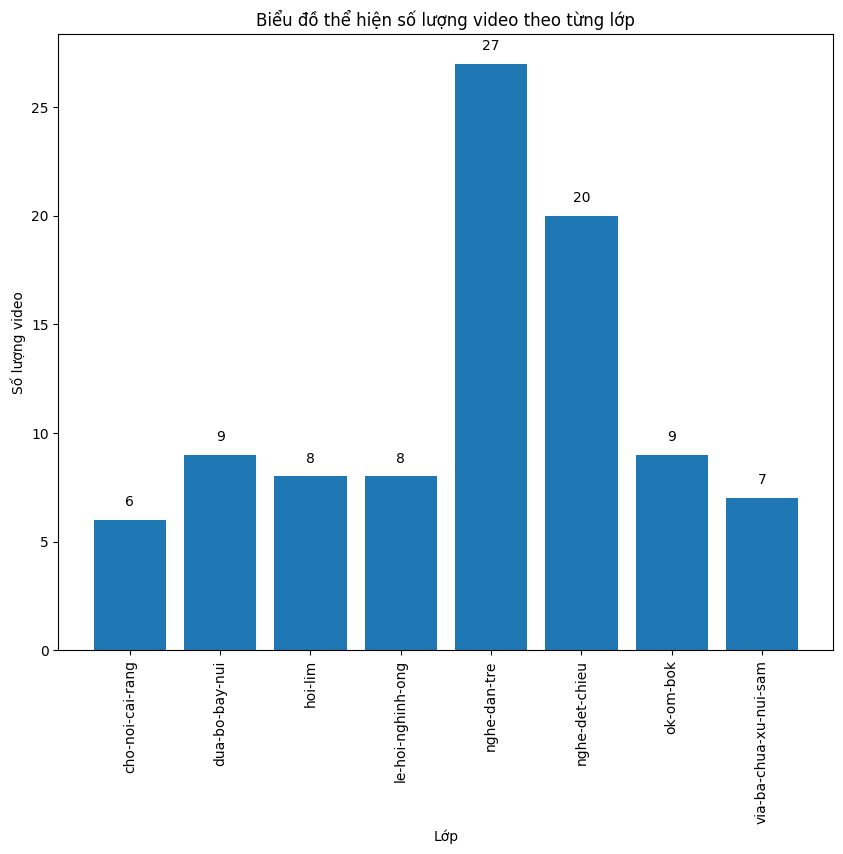
\includegraphics[width=\linewidth]{images/part-02/chap-02/sec-02/VideoNumber.png}
\caption{Số lượng video theo từng lớp}
\label{fig:VideoNumber}
\end{figure}